\documentclass[11pt, english]{article}
\usepackage{graphicx}
\usepackage[colorlinks=true, linkcolor=blue]{hyperref}
\usepackage[spanish]{babel}
\selectlanguage{english}
\usepackage[utf8]{inputenc}
\usepackage[svgnames]{xcolor}
\usepackage{booktabs}


\usepackage{listings}
\usepackage{afterpage}
\pagestyle{plain}

\definecolor{dkgreen}{rgb}{0,0.6,0}
\definecolor{gray}{rgb}{0.5,0.5,0.5}
\definecolor{mauve}{rgb}{0.58,0,0.82}

%\lstset{language=R,
%    basicstyle=\small\ttfamily,
%   stringstyle=\color{DarkGreen},
%    otherkeywords={0,1,2,3,4,5,6,7,8,9},
%    morekeywords={TRUE,FALSE},
%    deletekeywords={data,frame,length,as,character},
%    keywordstyle=\color{blue},
%    commentstyle=\color{DarkGreen},
%}

\lstset{frame=tb,
language=R,
aboveskip=3mm,
belowskip=3mm,
showstringspaces=false,
columns=flexible,
numbers=none,
keywordstyle=\color{blue},
numberstyle=\tiny\color{gray},
commentstyle=\color{dkgreen},
stringstyle=\color{mauve},
breaklines=true,
breakatwhitespace=true,
tabsize=3
}

\usepackage{here}


\textheight=21cm
\textwidth=17cm
%\topmargin=-1cm
\oddsidemargin=0cm
\parindent=0mm
\pagestyle{plain}

%%%%%%%%%%%%%%%%%%%%%%%%%%
% La siguiente instrucción pone el curso automáticamente%
%%%%%%%%%%%%%%%%%%%%%%%%%%

\usepackage{color}
\usepackage{ragged2e}

\global\let\date\relax
\newcounter{unomenos}
\setcounter{unomenos}{\number\year}
\addtocounter{unomenos}{-1}
\stepcounter{unomenos}
\gdef\@date{ Curso  2018 / \arabic{unomenos}}

\begin{document}

\begin{titlepage}

\begin{center}
\vspace*{-1in}
\begin{figure}[htb]
\begin{center}
\includegraphics[width=10cm]{../res/pics/logo.jpg}
\end{center}
\end{figure}

\vspace*{0.4in}
\begin{large}
\textsc{Procesadores de Lenguaje}:\\
\end{large}
\vspace*{0.2in}
\begin{Large}
\textbf{\textsc{Nombre de nuestro lenguaje}} \\
\end{Large}
\vspace*{0.3in}
\begin{large}
\@date\\
\end{large}
\vspace*{0.3in}
\rule{80mm}{0.1mm}\\
\vspace*{0.1in}
\begin{large}
Realizado por: \\

Medina Medina, David Alberto  \\
Brito Ramos, Christian  \\
Hernández Delgado, Christopher \\
López González, Néstor \\
\vspace*{0.3in}
\end{large}

\includegraphics[width=3cm]{../res/pics/LogoEscuela.jpg}
\end{center}
\end{titlepage}

\newcommand{\CC}{C\nolinebreak\hspace{-.05em}\raisebox{.4ex}{\tiny\bf +}\nolinebreak\hspace{-.10em}\raisebox{.4ex}{\tiny\bf +}}
\def\CC{{C\nolinebreak[4]\hspace{-.05em}\raisebox{.4ex}{\tiny\bf ++}}}

\tableofcontents
\newpage

\section{Definición del lenguaje (Autor: Quien termine antes)}\label{Introduction}
Introducir breve introducción del lenguaje que planteamos.
\newpage

\subsection{Tipos de datos (David)}\label{data-type}
Cualquier leguaje de programación necesita definir un conjunto de \emph{tipos de datos}, esto es, la batería de valores y operaciones que puede adquirir una variable. Cada tipo de dato está definido en el lenguaje por un \emph{literal} único que lo representa, lo que permite que cada tipo de dato tenga un representación física específica.

Los tipos de datos definidos en el lenguaje son los que figuran en el \emph{cuadro \ref{tab:table1}}. Las características críticas de implementación que define a cada tipo son:

\begin{description}
	\item[Entero] Representa a todas y cada una de las variables enteras que sean declaradas en el lenguaje. Este tipo de dato presenta un tamaño de 4 bytes (32 bits) y permite representar números enteros con signo. El \emph{complemento a 2} es el sistema elegido para definir el signo del número entero. Este dato se representa por el literal \texttt{int}. El rango de valores que puede tomar es 
	
	\begin{equation}\label{eq:equation1}
		\left [-2^{N-1},\: 2^{N-1}-1 \right ] = \left [-2^{32-1},\: 2^{32-1}-1 \right] = \left [-2147483648,\: 2147483647 \right]
	\end{equation}
	
	donde, $N$ es el número de bits disponibles para representar el número entero (32 bits).
	\item[Coma flotante de simple precisión] Este tipo de dato representa número reales en coma flotante de simple precisión con un tamaño de 4 bytes (32 bits) siguiendo el estándar \emph{IEEE 754}. En la figura \ref{fig:figure1} puede observarse como esta representación binaria los bits se organizan en tres sectores principales:
	\begin{itemize}
		\item \textbf{Signo} (1 bit). Se trata de un sólo bit que define el signo del número: positivo (0) o negativo (1).
		\item  \textbf{Exponente (8bits)}. Se trata de un número entero con signo de complemento a 2 ($\left [ -128,\: 127\right ]$)
		\item \textbf{Mantisa (23 bits)}. Conforma la fracción a la derecha de la coma binaria y un bit de encabezado implícito.
	\end{itemize}
	Este tipo de dato se representa con el literal \texttt{real}. Su rango de valores es de $\left [ 1.18 \cdot 10^{–38},\; 3.4 \cdot 10^{38} \right ]$.
	\begin{figure}[H]\label{fig:figure1}
		\centering
		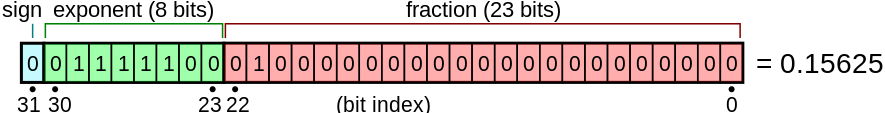
\includegraphics[width=0.75\textwidth]{../res/pics/data-types/float_diag.png}
		\caption{Representación binaria de número en coma flotante de simple precisión (\emph{IEEE 754})}
	\end{figure}

	\item[Caracter] Este tipo de dato es usado para representar caracteres de codificación \emph{UTF-8}, es por este motivo que el tamaño de que ocupan las variables de tipo caracter son de 1-4 bytes siendo \texttt{char} el literal que lo representa.
	\item[Booleano] Se trata de un tipo de dato utilizado para representar representar valores booleanos. Su tamaño es de 1 bit, por lo que tan solo puede tomar dos valores: \texttt{1} (verdadero) ó \texttt{0} (falso). El literal que lo representa es \texttt{bool}.
\end{description} 

\begin{table}[h!]
	\begin{center}
		\caption{Tipos de datos}
		\label{tab:table1}
		\begin{tabular}{l|l|l|l}
			\toprule
			\textbf{Tipo} & \textbf{Literal} & \textbf{Tamaño} & \textbf{Rango}\\
			\midrule
			Entero & int &4 Bytes & $\left [-2147483648,\: 2147483647 \right]$\\
			Coma flotante de simple precisión & real & 4 Byte & $\left [ 1.18 \cdot 10^{–38},\; 3.4 \cdot 10^{38} \right ]$\\
			Caracter & char & 1-4 Byte & $\left [ \texttt{0x00 - 0xFFFFFFFF} \right ]$\\
			Lógico & bool & 1 Bit & $\left [0,\; 1 \right ]$\\
			\bottomrule
		\end{tabular}
	\end{center}
\end{table}

En el siguiente ejemplo se muestra cómo se declaran las variables con los literales de los tipos descritos anteriormente:

\lstinputlisting[language=C++]{../res/lst/data-types/data-type.x}

\subsection{Colecciones de datos: \texttt{Arrays}}\label{arrays}
Las variables pueden ser agrupadas en colecciones de datos de una dimensión denominados \texttt{arrays}. En este lenguaje, cualquier tipo de dato puede formar parte de un \texttt{array}.

Para declarar un \texttt{array} del tipo que se desee, debe usar la gramática \ref{grammar:1.2.1}:
	\begin{equation}\label{grammar:1.2.1}
		tipo[<int>]\; nombre\_variable
	\end{equation}

donde el $tipo$ define el tipo de dato e $<int>$ un valor entero opcional que define el tamaño del \texttt{array}. Cuando no se indica este último valor entero, no se lleva a término la reserva en memoria del \texttt{array} declarado. En caso contrario, se reservará en memoria tantos bytes/bits como fueren necesarios para generar una colección de tipos de datos del tamaño indicado por $<int>$. El número de bytes/bits a reservar está determinado por el tipo de dato y el tamaño del \texttt{array},
	\begin{equation}\label{eq:1.2}
		Tamaño_{memoria} = Tamaño_{tipo\, dato} \times Tamaño_{array}
	\end{equation}

Un \texttt{array} que ha sido declarado con anterioridad puede ser redefinido haciendo uso de la gramática \ref{grammar:1.2.2},
	\begin{equation}\label{grammar:1.2.2}
	tipo[ \, ]\; nombre\_variable = new\; tipo[<int>]\; \{ \\
	expresion\_1, expresion\_2, ...\;\}
	\end{equation}

Esta notación es alternativa a la gramática \ref{grammar:1.2.1}, donde podremos inicializar el \texttt{array} a un conjunto de expresiones separados por comas encerrados dentro de los caracteres \texttt{\{} y \texttt{\}}. Estas expresiones son opcionales. El tamaño máximo del vector y, por tanto, de expresiones es el indicado por $<int>$ el cual es un número entero de caracter obligatorio.

Si se declara un \texttt{array} utilizando la gramática \ref{grammar:1.2.1} o \ref{grammar:1.2.2} sin expresiones en esta última, el array es inicializado en todas sus posiciones al valor \texttt{0} para tipos de datos enteros y reales. Para caracteres el valor por defecto es el caracter \texttt{nulo}. Y para tipos booleanos el valor por defecto es \texttt{FALSE}.

La gramática \ref{grammar:1.2.3} es necesaria para acceder al valor de un elemento del \texttt{array} en una posición arbitraria del mismo,
	\begin{equation}\label{grammar:1.2.3}
	nombre\_variable\; [<int>]
	\end{equation}
donde $<int>$ es un entero obligatorio que indica la posición del \texttt{array} a la que se desea acceder.

El \texttt{array} de caracteres constituyen los denominados \texttt{string}, los cuales requieren una atención especial ya que es posible cargar una variable con una secuencia de caracteres sin ser necesaria la declaración dada por la gramática \ref{grammar:1.2.2}. La gramática \ref{grammar:1.2.4} define la instancia de un \texttt{string} con un conjunto de caracteres localizados entre los caracteres comillas doble,

	\begin{equation}\label{grammar:1.2.4}
	nombre\_variable\; = " <char><char>..."
	\end{equation}

El siguiente listado muestra algunos ejemplos de uso de los \texttt{array} definidos en este lenguaje:

\lstinputlisting[language=C++]{../res/lst/array/array.x}

\subsection{Palabras reservadas (Christian)}\label{keywords}
Aquí va el texto. Poner siempre un código de ejemplo.
\newpage

\subsection{Comentarios (Christian)}\label{commentaries}
Aquí va el texto. Poner siempre un código de ejemplo.
\newpage

\subsection{Tipos de operadores}\label{operators}
Aquí va el texto. Poner siempre un código de ejemplo.

\subsubsection{Operadores aritméticos (David)}\label{arithmetic-operators}
Aquí va el texto. Poner siempre un código de ejemplo.

\subsubsection{Operadores lógicos (Néstor)}\label{logical-operators}
Aquí va el texto. Poner siempre un código de ejemplo.

\subsubsection{Operadores bit a bit (Christian)}\label{bitwise-operators}
Aquí va el texto. Poner siempre un código de ejemplo.

\subsubsection{Operadores de array (Christopher)}\label{array-operators}
Aquí va el texto. Poner siempre un código de ejemplo.
\newpage

\subsection{Estructuras de control}
Aquí va el texto. Poner siempre un código de ejemplo.

\subsubsection{Sentencias \texttt{if-ifelse-else} (Néstor)}\label{if}
Aquí va el texto. Poner siempre un código de ejemplo.

\subsubsection{Bucle \texttt{for-forelse-else} (Christopher)}\label{for}
Aquí va el texto. Poner siempre un código de ejemplo.

\subsubsection{Bucle \texttt{while-whileelse-else} (Christian)}\label{while}
Aquí va el texto. Poner siempre un código de ejemplo.
\newpage

\subsection{Funciones (David)}\label{functions}
Aquí va el texto. Poner siempre un código de ejemplo.
\newpage

\subsection{Funciones primitivas (Néstor)}\label{primitive-functions}
Aquí va el texto. Poner siempre un código de ejemplo.
\newpage

\subsection{Código ejemplo (Christopher)}\label{example-code}
Aquí va el código de ejemplo con el que probaremos nuestro compilador.

\end{document}